\section{Position and Orientation}
\subsection{Introduction}
Kinematics studies the movement of an object -- in our case of a robot -- without taking into acount the forces generating it. Instead, it only handles aspects such as position, orientation, speed and momentum of bodies in movement.

Consider for instance a robotic arm. We can design a simplified scheme of the robot and its environment, to create a kinematic pipeline and reference frames associated to each of these objects.

\begin{figure}[H]
    \centering
    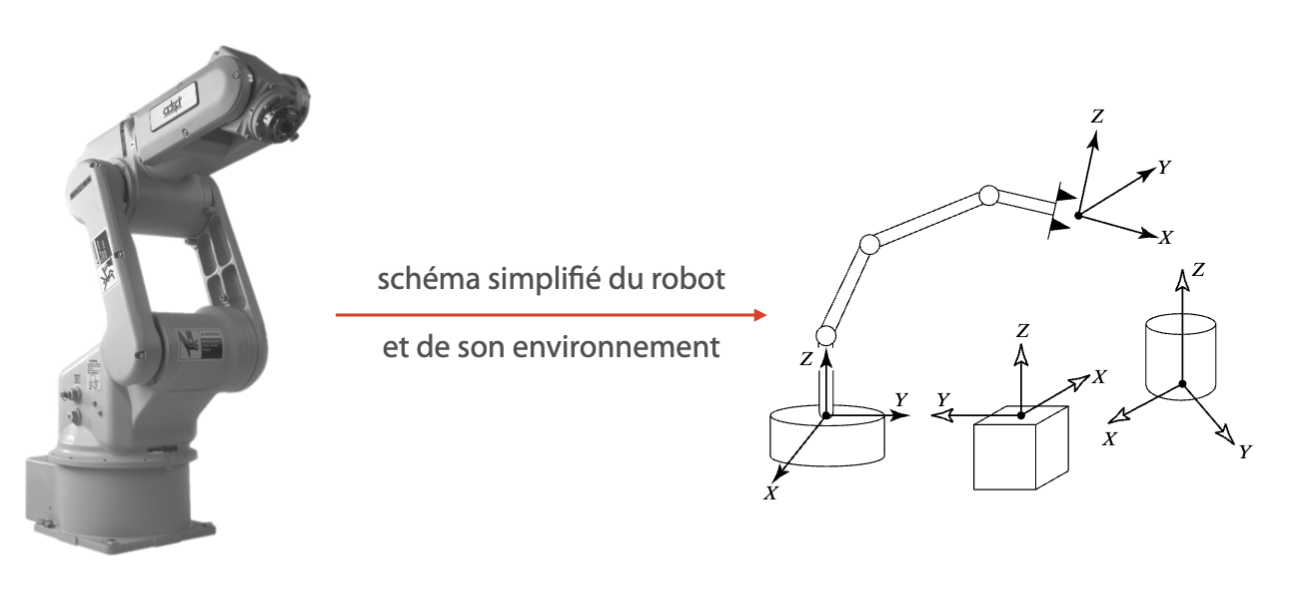
\includegraphics[width=.6\textwidth]{position/arm-scheme.png}
    \caption{Simplified scheme of the robot feature the kinematic pipeline and reference frames.}
\end{figure}

\emph{Direct kinematics} allows to compute the position and orientation of the terminal organ given, for instance, the angles of the articulations.

\begin{figure}[H]
    \centering
    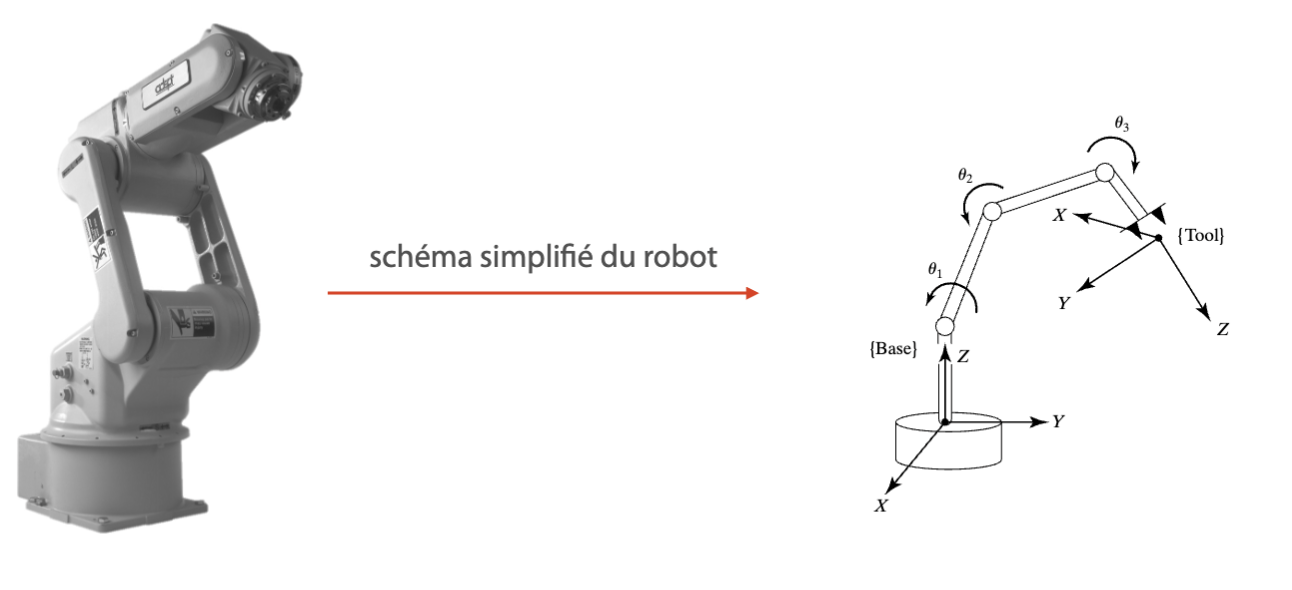
\includegraphics[width=.6\textwidth]{position/direct-kinematic.png}
\end{figure}

\emph{Invert kinematics} answers the question the other way around: given the position and orientation of a boyd, how can we compute the values of the articulations angles. Invert kinematics is used for instance for trajectory tracking: given a reference trajectory, how can we compute the speed of the articulations?

\subsection{Points, frames and transformations}
\subsubsection{Position of a point in space}
Once that a frame of reference $\{A\}$ is defined, we can localize any point of the universe given a \emph{position vector}:
\begin{figure}[H]
    \centering

    \begin{minipage}{0.4\textwidth}
        \begin{equation*}
            \prescript{A}{}{P} = \begin{bmatrix}
                p_x \\ p_y \\ p_z
            \end{bmatrix}
        \end{equation*}
    \end{minipage}
    \begin{minipage}{0.4\textwidth}
        \centering
        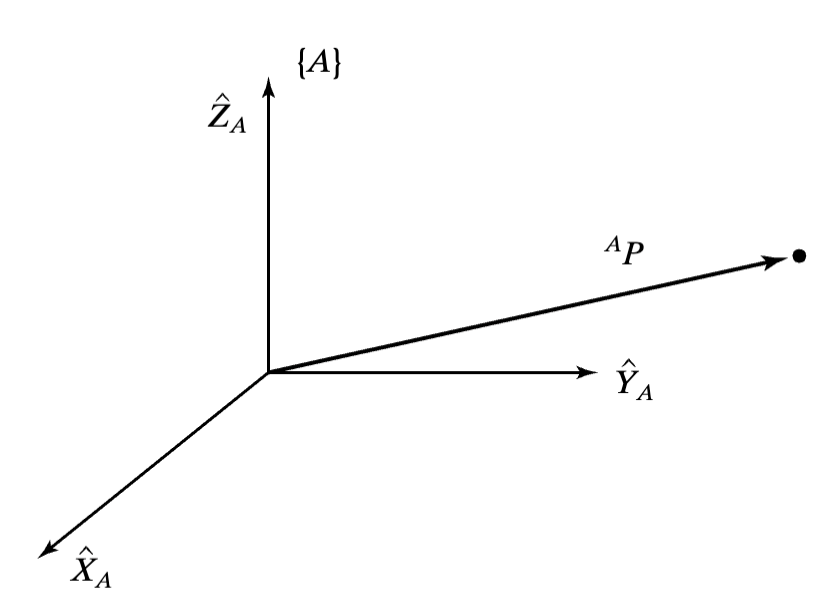
\includegraphics[width=.8\textwidth]{position/position-frame.png}
    \end{minipage}
    \caption{Vector and position of the point established in the frame $\{A\}$.}
\end{figure}

\subsubsection{Position and orientation of a body in space}
To define the orientation of a body in space, we need to define a frame of reference $\{B\}$ attached to this body. The orientation is therefore defined as the expression of this coordinate system in the reference frame $\{A\}$.
\begin{figure}[H]
    \centering

    \begin{minipage}{0.5\textwidth}
        \begin{equation*}
            \prescript{A}{B}{R} = \begin{bmatrix}
                \prescript{A}{}{\hat{X}}_B & \prescript{A}{}{\hat{Y}}_B & \prescript{A}{}{\hat{Z}}_B
            \end{bmatrix}
            = \begin{bmatrix}
                r_{11} & r_{12} & r_{13} \\
                r_{21} & r_{22} & r_{23} \\
                r_{31} & r_{32} & r_{33}
            \end{bmatrix}
        \end{equation*}
    \end{minipage}
    \begin{minipage}{0.4\textwidth}
        \centering
        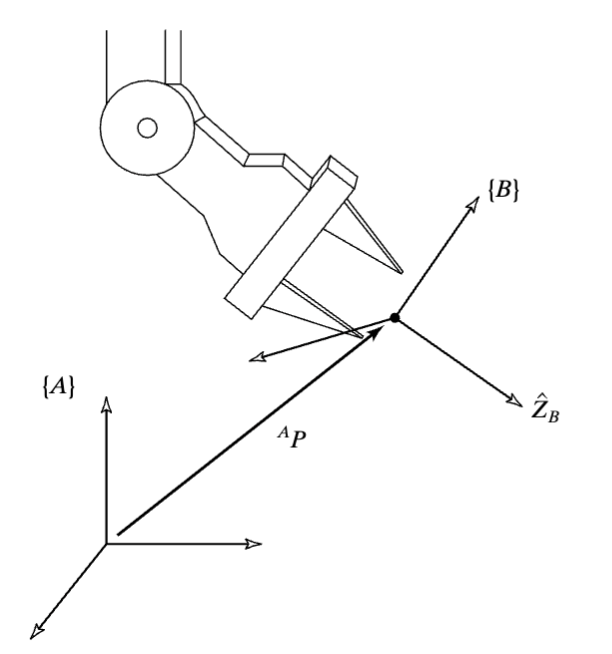
\includegraphics[width=.8\textwidth]{position/body-orientation.png}
    \end{minipage}
    \caption{Expression of the coordinate system $\{B\}$ in the reference frame $\{A\}$, and the associated position and orientation of the body.}
\end{figure}
Each element of the matrix $\prescript{A}{B}{R}$ is the scalar product between the vectors of the two coordinate systems $\{B\}$ and $\{A\}$:
\begin{equation*}
    \prescript{A}{B}{R} = \begin{bmatrix}
        \prescript{A}{}{\hat{X}}_B & \prescript{A}{}{\hat{Y}}_B & \prescript{A}{}{\hat{Z}}_B
    \end{bmatrix}
    = \begin{bmatrix}
        \hat{X}_B\cdot\hat{X}_A & \hat{Y}_B\cdot\hat{X}_A & \hat{Z}_B\cdot\hat{X}_A \\
        \hat{X}_B\cdot\hat{Y}_A & \hat{Y}_B\cdot\hat{Y}_A & \hat{Z}_B\cdot\hat{Y}_A \\
        \hat{X}_B\cdot\hat{Z}_A & \hat{Y}_B\cdot\hat{Z}_A & \hat{Z}_B\cdot\hat{Z}_A
    \end{bmatrix}
\end{equation*}
The lines correspond to the axes of the frame $\{A\}$ expressed in the frame $\{B\}$. Note that the invert of a rotation matrix is its transpose:
\begin{equation*}
    \prescript{A}{B}{R}^T = \prescript{A}{B}{R}^{-1} = \prescript{B}{A}{R}
\end{equation*}

\subsubsection{Rotation matrices}
We showed that the orientation of the body in space could be expressed as a 3-dimensional rotation matrix. The group of 3-dimensional rotation matrices is denoted $\SO(3)$, and is composed of all the matrices that are orthonormal, that is orthogonal and with a determinant equal to 1:
\begin{equation*}
    \SO(3) = \set{R\in\mathcal{M}_{3}(\R)}{RR^T=I_3 \text{ and } \det(R) = +1}
\end{equation*}
If we write:
\begin{equation*}
    R = \begin{bmatrix}
        \hat{X} & \hat{Y} & \hat{Z}
    \end{bmatrix}
\end{equation*}
Then $R\in\SO(3)$ if and only if:
\begin{equation*}
    \begin{cases}
        \hat{X}\cdot\hat{Y} = 0 \\
        \hat{Y}\cdot\hat{Z} = 0 \\
        \hat{Z}\cdot\hat{X} = 0 \\
    \end{cases}
    \quad\text{and}\quad
    \begin{cases}
        \hat{X}\cdot\hat{X} = 1 \\
        \hat{Y}\cdot\hat{Y} = 1 \\
        \hat{Z}\cdot\hat{Z} = 1 \\
    \end{cases}
\end{equation*}
Note that we have 9 degrees of freedom and 6 independent constraints, so the group $\SO(3)$ is 3-dimensional.

\subsection{Rotation representations}
There are several ways to represent a rotation matrix, each with its own advantages and drawbacks. The most common representations are:
\begin{itemize}
    \item Orthonormal 3 by 3 matrices --- 9 components
    \item Euler angles --- 3 components
    \item Axis-angle representation --- 3 components
    \item Quaternions --- 4 components
\end{itemize}

\subsubsection{Euler angles}